% --------------------------------------------------------------------------- %
% Poster for the ECCS 2011 Conference about Elementary Dynamic Networks.      %
% --------------------------------------------------------------------------- %
% Created with Brian Amberg's LaTeX Poster Template. Please refer for the     %
% attached README.md file for the details how to compile with `pdflatex`.     %
% --------------------------------------------------------------------------- %
% $LastChangedDate:: 2011-09-11 10:57:12 +0200 (V, 11 szept. 2011)          $ %
% $LastChangedRevision:: 128                                                $ %
% $LastChangedBy:: rlegendi                                                 $ %
% $Id:: poster.tex 128 2011-09-11 08:57:12Z rlegendi                        $ %
% --------------------------------------------------------------------------- %
\documentclass[a0paper,portrait, fontscale=0.285]{baposter}
\usepackage{relsize}		% For \smaller
\usepackage{url}			% For \url
\usepackage{epstopdf}	% Included EPS files automatically converted to PDF to include with pdflatex
\usepackage{lipsum}	% generate non sense text to fill boxes

%%% Global Settings %%%%%%%%%%%%%%%%%%%%%%%%%%%%%%%%%%%%%%%%%%%%%%%%%%%%%%%%%%%

\graphicspath{{pix/}}	% Root directory of the pictures
\tracingstats=2			% Enabled LaTeX logging with conditionals

%%% Color Definitions %%%%%%%%%%%%%%%%%%%%%%%%%%%%%%%%%%%%%%%%%%%%%%%%%%%%%%%%%

\definecolor{bordercol}{RGB}{40,40,40}
\definecolor{headercol1}{RGB}{186,215,230}
\definecolor{headercol2}{RGB}{80,80,80}
\definecolor{headerfontcol}{RGB}{0,0,0}
\definecolor{boxcolor}{RGB}{255,255,255} % white

%%%%%%%%%%%%%%%%%%%%%%%%%%%%%%%%%%%%%%%%%%%%%%%%%%%%%%%%%%%%%%%%%%%%%%%%%%%%%%%%
%%% Utility functions %%%%%%%%%%%%%%%%%%%%%%%%%%%%%%%%%%%%%%%%%%%%%%%%%%%%%%%%%%

%%% Save space in lists. Use this after the opening of the list %%%%%%%%%%%%%%%%
\newcommand{\compresslist}{
	\setlength{\itemsep}{1pt}
	\setlength{\parskip}{0pt}
	\setlength{\parsep}{0pt}
}

%%%%%%%%%%%%%%%%%%%%%%%%%%%%%%%%%%%%%%%%%%%%%%%%%%%%%%%%%%%%%%%%%%%%%%%%%%%%%%%
%%% Document Start %%%%%%%%%%%%%%%%%%%%%%%%%%%%%%%%%%%%%%%%%%%%%%%%%%%%%%%%%%%%
%%%%%%%%%%%%%%%%%%%%%%%%%%%%%%%%%%%%%%%%%%%%%%%%%%%%%%%%%%%%%%%%%%%%%%%%%%%%%%%

\begin{document}
\typeout{Poster rendering started}

%%% Setting Background Image %%%%%%%%%%%%%%%%%%%%%%%%%%%%%%%%%%%%%%%%%%%%%%%%%%
%\background{
%	\begin{tikzpicture}[remember picture,overlay]%
%	\draw (current page.north west)+(-2em,2em) node[anchor=north west]
%	{\includegraphics[height=1.1\textheight]{figures/background}};
%	\end{tikzpicture}
%}

%%% General Poster Settings %%%%%%%%%%%%%%%%%%%%%%%%%%%%%%%%%%%%%%%%%%%%%%%%%%%
%%%%%% Eye Catcher, Title, Authors and University Images %%%%%%%%%%%%%%%%%%%%%%
\begin{poster}{
	grid=false,
	%columns=5,
	% Option is left on true though the eyecatcher is not used. The reason is
	% that we have a bit nicer looking title and author formatting in the headercol
	% this way
	%eyecatcher=false,
	borderColor=bordercol,
	headerColorOne=blue!20,
	headerColorTwo=blue!20,
	headerFontColor=headerfontcol,
	% Only simple background color used, no shading, so boxColorTwo isn't necessary
	boxColorOne=boxcolor,
	headershape=roundedright,
	headerfont=\Large\sf\bf,
	textborder=rectangle,
	headerborder=open,
  	boxshade=plain,
	background=shadetb,
	bgColorOne=white,
	bgColorTwo=blue!10,
	headerheight=7cm
}
%%% Eye Cacther %%%%%%%%%%%%%%%%%%%%%%%%%%%%%%%%%%%%%%%%%%%%%%%%%%%%%%%%%%%%%%%
{
	%\includegraphics[width=4cm]{figures/it-logo.png}
}
%%% Title %%%%%%%%%%%%%%%%%%%%%%%%%%%%%%%%%%%%%%%%%%%%%%%%%%%%%%%%%%%%%%%%%%%%%
{\sf\bf
	MitoBench: An interactive visual workbench for population genetics on mitochondrial DNA
}
%%% Authors %%%%%%%%%%%%%%%%%%%%%%%%%%%%%%%%%%%%%%%%%%%%%%%%%%%%%%%%%%%%%%%%%%%
{
	\vspace{1em} Judith Neukamm$^{1,3*}$, Alexander Peltzer$^{1,2,3*}$, Wolfgang Haak$^{2}$, Johannes Krause$^{1,2}$ and Kay Nieselt$^{3}$\\
	\vspace{1em}
	{\footnotesize 	1 Institute for Archaeological Sciences, Archaeo- and Paleogenetics, University of Tuebingen, Germany.\\
	2 Max Planck Institute for the Science of Human History, Jena, Germany.\\
	3 Integrative Transcriptomics, Center for Bioinformatics (ZBIT), University of Tuebingen, Germany.\\
	$*$These authors contributed equally to the study.
	}
}
%%% Logo %%%%%%%%%%%%%%%%%%%%%%%%%%%%%%%%%%%%%%%%%%%%%%%%%%%%%%%%%%%%%%%%%%%%%%
{
% The logos are compressed a bit into a simple box to make them smaller on the result
% (Wasn't able to find any bigger of them.)
\setlength\fboxsep{0pt}
\setlength\fboxrule{0.5pt}
	%\fbox{
		\begin{minipage}{14em}
			\includegraphics[width=4cm]{figures/it-logo.png}\\
			\\
			\includegraphics[width=4cm]{figures/mpi-logo.png}
		\end{minipage}
	%}
}



%----------------------------------------------------------------------------------------
%	Introduction
%----------------------------------------------------------------------------------------

\headerbox{Introduction}{name=introduction, row=0, column=0, span=3}{

Despite the availability of modern next generation sequencing technologies and
therefore nuclear human genomes, the sequencing and analysis of mitochondrial DNA
(mtDNA) is still common. Especially in the research field of ancient DNA and the
context of population genetics, mtDNA is often the only proxy available to study
extinct populations and their relationship with modern populations. As a consequence,
many population genetic studies rely on the analysis of mtDNA. \\
A plethora of methods for the analysis of mtDNA exist, that address questions in
population genetics, phylogeny and others. However, these tools typically rely on
different file formats and often require manual interaction with the data for downstream
analysis. Ultimately, these steps can be cumbersome, especially for non-bioinformaticians,
resulting in an increased risk of errors during the analysis. \\
To tackle these issues, we present MitoBench, a workbench to interactively analyze
and visualize mitochondrial genomes with a focus on population genetics. The
graphical user interface is kept simple, to accommodate even users without further
prior knowledge on computational methods. Furthermore, it shows additional
information such as metadata and statistics. Currently, MitoBench offers automatic
file conversion tools to connect the workbench with existing analysis methods
such as BEAST, Arlequin and others.

}



%----------------------------------------------------------------------------------------
%	MitoDB
%----------------------------------------------------------------------------------------

\headerbox{MitoDB}{name=mitodb, row=1, column=1, span=2, below=introduction}{
	\begin{itemize}
		\item Web-Frontend with Vaadin Java Framework
		\item Backend with PostgreSQL, providing sequence information and meta-data (SQL)
		\item Curated data upload with metadata
		\item Retrieval possible through WebUI and mitoBench
	\end{itemize}
}


%----------------------------------------------------------------------------------------
%  Workflow
%----------------------------------------------------------------------------------------


\headerbox{Workflow}{name=workflow, column=0, below=introduction, bottomaligned=mitodb}{
\begin{center}
		\includegraphics[width=0.67\textwidth]{figures/workflow_yed.jpg}
\end{center}
}




%----------------------------------------------------------------------------------------
%	References
%----------------------------------------------------------------------------------------

\headerbox{References}{name=references, column=0, span=2, above=bottom}{
	\footnotesize
	\begingroup
	\renewcommand{\section}[2]{}%
	\bibliography{sample}
	\endgroup
}




%----------------------------------------------------------------------------------------
%	Contact
%----------------------------------------------------------------------------------------

\headerbox{Contact}{name=contact, column=2, aligned=references,above=bottom}{
	\begin{description}\compresslist
		\item Judith Neukamm
		\item University of T\"ubingen
		%\item[Web] www.university.edu/smithlab
		\item[Email] judith.neukamm@uni-tuebingen.de
		\item[Phone] +49 7071 2975651
	\end{description}
}



%----------------------------------------------------------------------------------------
%	Conclusions
%----------------------------------------------------------------------------------------

\headerbox{Conclusions}{name=conclusions,row=0, column=2,  below=mitodb, above=references}{
	\textbf{MitoBench}
	\begin{itemize}
		\item Easy file handling and file conversion
		\item Combination, manipulation and visualization of mitochondrial data
		\item Multiple filtering options
		\item Statistics
	\end{itemize}
	\textbf{MitoDB}
	\begin{itemize}
		\item Collection of mitochondrial data plus meta information
		\item Curated database
	\end{itemize}
}




%----------------------------------------------------------------------------------------
%	Mitobench
%----------------------------------------------------------------------------------------


\headerbox{MitoBench}{name=mitobench, column=0, span=2, below=workflow, bottomaligned=conclusions}{
\begin{minipage}[t]{0.5\textwidth}
	\textbf{Data import and export}
	%\begin{itemize}
%		\item (Multi-) FastA 
%		\item ARP (Arlequin format \cite{excoffier2010arlequin})
%		\item HSD (Haplogrep 2 format \cite{weissensteiner2016haplogrep}) 
%		\item Excel file 
%		\item Generic formats (tsv/csv format) 
%	\end{itemize}	
\begin{center}
	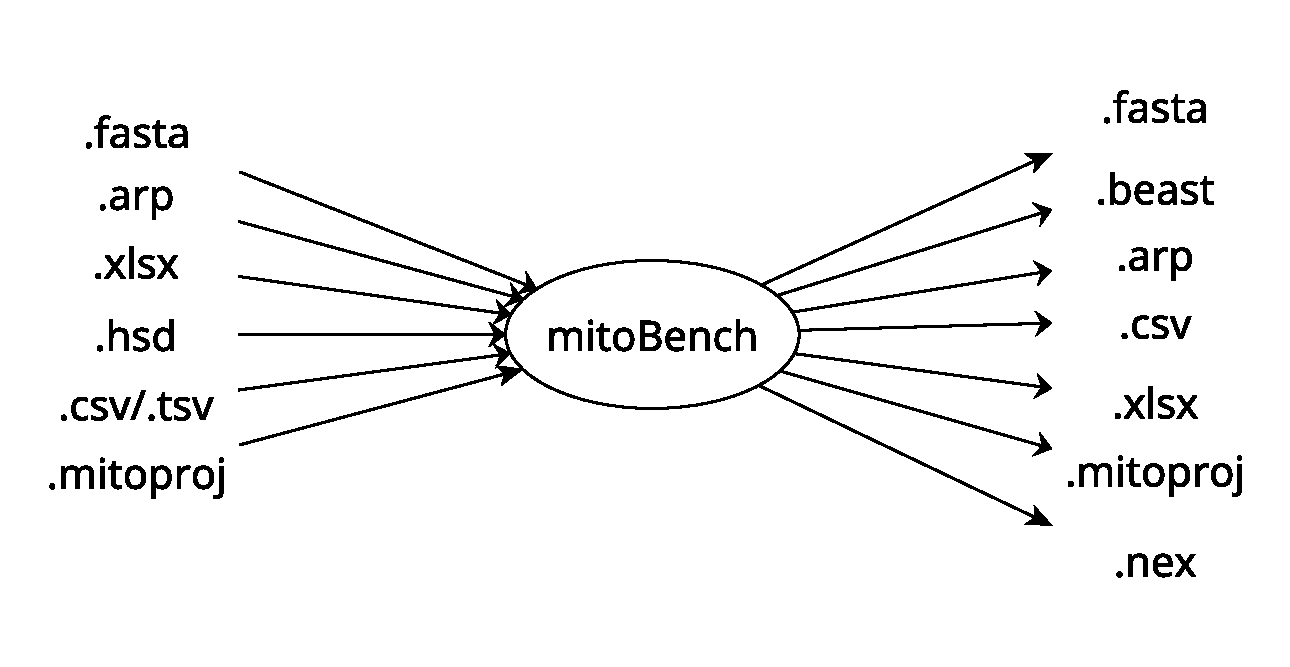
\includegraphics[width=0.8\textwidth]{figures/import_export.jpg}
	\end{center}
\end{minipage}
\hspace{0.5em}
\begin{minipage}[t]{0.5\textwidth}
\textbf{Data representation}
\begin{center}
		\includegraphics[width=0.8\textwidth]{figures/load_generic.png}
\end{center}
\end{minipage}

\vspace{1em}

\begin{minipage}[t]{0.5\textwidth}
\textbf{	Data grouping}
	\begin{itemize}
		\item interested in behaviour of different groups\\
		$\rightarrow$ Group data by feature 
		\item internal grouping (columns not sorted)
	\end{itemize}
\end{minipage}
\hspace{0.5em}
\begin{minipage}[t]{0.5\textwidth}
\textbf{Data filtering / Statistics}
	\begin{itemize}
		\item Haplogroup filtering
		\item Filtering based on Mutation
		\item Haplogroup frequencies
		\item Mutation frequencies
	\end{itemize}
\end{minipage}

\vspace{1em}

\begin{minipage}[t]{0.5\textwidth}
\textbf{Data visualization}
\begin{center}
		\includegraphics[width=0.8\textwidth]{figures/stackedBarchart.png}
\end{center}
\end{minipage}
\hspace{0.5em}
\begin{minipage}[t]{0.5\textwidth}
\textbf{Data visualization}
	\begin{center}
		\includegraphics[width=0.8\textwidth]{figures/profile.png}
	\end{center}
\end{minipage}

}




\end{poster}
\end{document}
